\documentclass[12pt]{article}
\usepackage{graphicx} % Required for inserting images
\usepackage{enumitem}
\usepackage{amsmath}
\usepackage{gvv-book}
\usepackage{gvv}

\title{\textbf{1.4.19}}
\author{\textbf{ee25btech11004 - Aditya Appana}}
\date{August 24, 2025}

\begin{document}

\maketitle

\section{Question}


Find the position vector of a point \textbf{R} which divides the line joining two points \textbf{P} and \textbf{Q} whose position vectors are $ \hat{i} + 2\hat{j} - \hat{k}$ and $-\hat{i} + \hat{j} + \hat{k} $ respectively in the ratio \textbf{2:1}
\begin{enumerate}[label=(\alph*)]
    \item externally
    \item internally   
\end{enumerate}

\section{Solution}

Given vector $\mathbf{P}$ is \begin{align} \myvec{ 1 \\ 2\\ -1}\end{align} and vector $\mathbf{Q}$ is \begin{align}\myvec{ -1 \\ 1 \\ 1 }\end{align} . \\

We need to find the points which divide line segment $\mathbf{PQ}$ internally and externally in the ratio \textbf{2:1}. \\



Let the point which divides $\mathbf{PQ}$ internally be $\mathbf{R}$. \\

Let the point which divides $\mathbf{PQ}$ externally be $\mathbf{S}$. \\

The formula to calculate the coordinates of the point which divides a line segment internally in the ratio m:n is 



\begin{align}
    \mathbf{R}=\frac{\frac{m}{n}\mathbf{P}+\mathbf{Q}}{\frac{m}{n}+1}
\end{align}

and to calculate the coordinates of the point which divides a line segment externally in the ratio m:n is 

\begin{align}
    \mathbf{S}=\frac{\frac{m}{n}\mathbf{P}-\mathbf{Q}}{\frac{m}{n}-1}
\end{align}

Substituting $P\myvec{ 1 \\ 2\\ -1}$ and $Q\myvec{ -1 \\ 1\\ 1}$ in the first formula, we get \vspace{0.5cm}

\begin{align}
    \mathbf{R}=\frac{2\myvec{ 1 \\ 2\\ -1}+\myvec{ -1 \\ 1\\ 1}}{\frac{2}{1}+1} = \frac{\myvec{ 2-1 \\ 4+1\\ -2+1}}{3} = \myvec{ 1/3\\ 5/3\\ -1/3}
\end{align}

\vspace{1cm}

Substituting $P\myvec{ 1 \\ 2\\ -1}$ and $Q\myvec{ -1 \\ 1\\ 1}$ in the second formula, we get  \vspace{0.5cm}

\begin{align}
    \mathbf{S}=\frac{2\myvec{ 1 \\ 2\\ -1}-\myvec{ -1 \\ 1\\ 1}}{\frac{2}{1}-1} = \frac{\myvec{ 2-(-1) \\ 4-1\\ -2-1}}{1} = \myvec{ 3\\ 3\\ -3}
\end{align}

\begin{figure}[H]
    \centering
    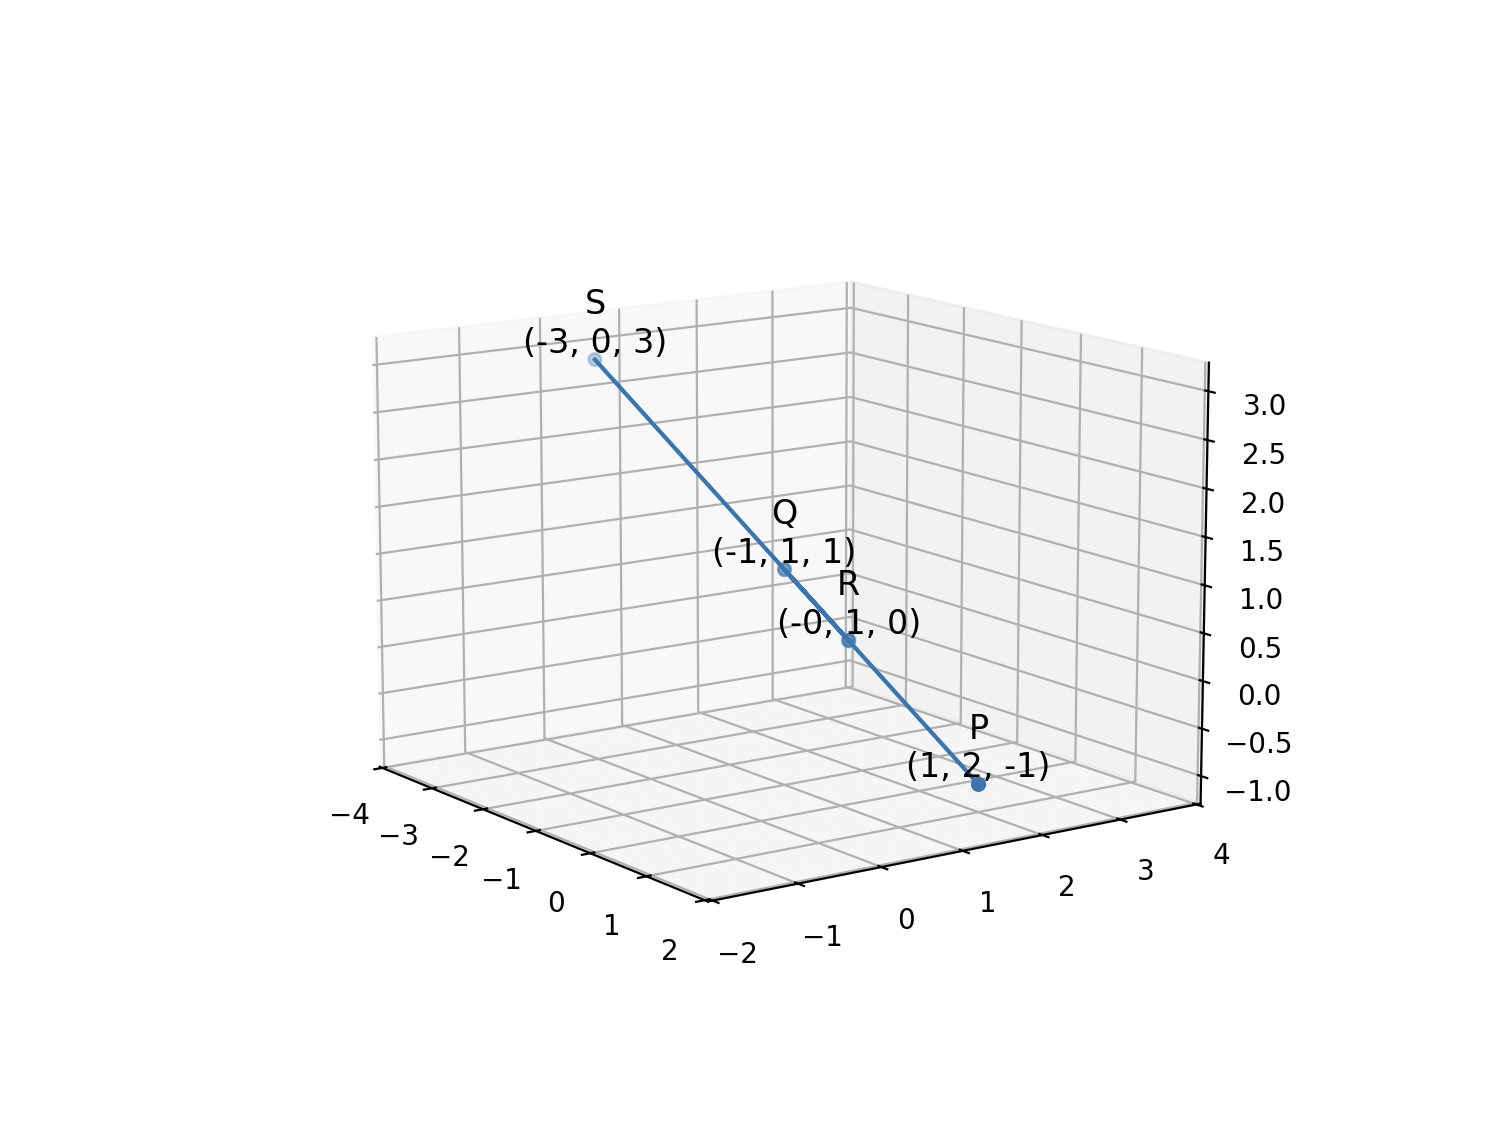
\includegraphics[width=1.1\columnwidth]{Figs/Figure_1.png}
    \caption{3D Plot}
    \label{fig:placeholder}
\end{figure}



\end{document}
